\chapter{Related Work}
\label{cha:relatedwork}

\section{OAuth 2.0 and OpenID Connect}
\label{cha:relatedwork:oauth}
%TODO: fix citing

Oauth is an open standard for access delegation, 
commonly used as a way for users to grant client applications access to their information on other applications.
Oauth was born as a necessary security measure, to avoid sharing plaintext credentials between applications.
Plaintext credential sharing, as outlined in \cite{rfcOauth2} has many security risks:

\begin{enumerate}
  \item Applications are forced to implement password authentication, to support the sharing of plaintext credentials.
  \item Third party applications gain overly broad access to the user's account.
  \item Users cannot revoke access to specific third party applications.
  \item If any of the third party applications are compromised, the user's account is at risk.
\end{enumerate}

Oauth adresses these issues by decoupling the client application from the role of the resource owner,
meaning that the client application will not get a full set of permissions to the user's account.
Insetead of handing his crendentials to the third party application,
the resource owner signs in, in the application's website which then issues an access token to the client application.
This method avoids the user having to share his credentials with third party applications.

\subsection{OAuth 2.0 Roles}

Oauth 2.0 defines four roles for participants in the protocol flow:

%TODO: rewrite this, it is looking too much like the original spec
\begin{enumerate}
  \item Resource owner: The entity that can grant access to a protected resource, typically this would be an end user of a web application.
  \item Resource server: The server hosting the protected resources.
  \item Client: The application requesting access to the protected resources. 
    OAuth 2.0 distinguishes between two types of clients: confidential and public clients.
    Confidential clients are capable of keeping their credentials confidential, while public clients, like browser-based applications, cannot.
  \item Authorization server: The server that issues access tokens to the client after the resource owner has been succesfully authenticated.
\end{enumerate}

The resource server and the authorization server can be the same entity, but they are not required to be.

\subsection{Authorization Grants}

%TODO: public and private client
%TODO: authorization tokens

Authorization Grants are credentials that are issued to clients, which can be exchanged for an access token.
This access token can be used to access the protected resources on the resource server.
Oauth 2.0 defines four authorization grants with different flows.

%TODO: footnote for http redirects or smthing

\subsubsection{Implicit}
\label{cha:relatedwork:oauth:implicit}

% The implicit grant is a simplified version of the Authorization Code grant.
The implicit grant is very helpful for public clients, as it doesn't require confidential client credentials.
This is very helpful for browser-based clients, as they can't store confidential credentials securely.
In the implicit grant users are redirected to the authorization server, where they authenticate thmeselves and authorize the client.
Afterwhich the authorization server issues an access token directly to the client,
this is done so with a HTTP redirect, where the access token is embedded in the redirect URL,
this way the client can extract the access token from the URL.
% The access token gets embedded in the redirect URL, after the resource owner was authenticated, which is then sent to the client.

In this flow the resource owner only authenticates with the authorization server, 
thus never having to share his credentials with the client.

Implicit grants have many security risks, as the access token is exposed in the URL and can be intercepted by a malicious attacker.
This is why PKCE (Proof Key for Code Exchange) was later introduced as an addition to the implicit grant \cite{rfcPkce}.

\subsubsection{Resource Owner Password Credentials}
\label{cha:relatedwork:oauth:passwordcredentials}

This grant type requires the resource owner to share his password credentials with the client.
The resource owner's password credentials represent an authorization grant,
which the client can exchange them for an access token.
Even though this grant type requires the resource owner to share his credentials with the client,
these are only used for one request and don't have to be stored.


\subsubsection{Client Credentials}
\label{cha:relatedwork:oauth:cleintcredentials}

The client credentials grant is used when the client is the resource owner.
Clients are typycally issued crendentials, which they can use to authenticate themselves.
Clients send these credentials to the authorization server and are issued an access token.

\subsubsection{Authorization Code}
\label{cha:relatedwork:oauth:authcode}

The Authorization Code grant is the most common grant type used in OAuth 2.0,
it is similar to the implicit grant \ref{cha:relatedwork:oauth:implicit}, as it also uses HTTP redirects and it doesn't require the resource owner to share his credentials with the client.
In the authorization code grant, the client redirects the resource owner to the authorization server.
There the resource owner authenticates himself and authorizes the client.
afterwhich the authorization server redirects the resource owner back to the client with an authorization code.
The client then authenticates itself with his confidential credentials on the authorization server and exchanges the authorization code for an access token.
As the client needs confidential credentials, this flow is only suitable for confidential clients.
The exact steps are shown in figure \ref{fig:oauth:authcodeflow}.

\begin{figure}[H]
    \centering
    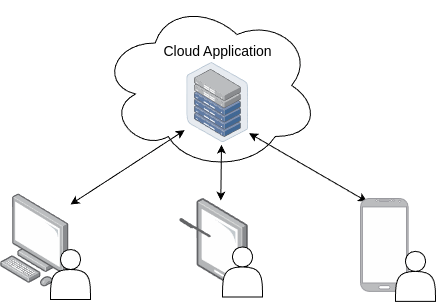
\includegraphics[scale=0.4]{images/basic-cloud-services.drawio.png}
    \caption{Cloud Application.}
    \label{fig:oauth:authcodeflow}
\end{figure}

\section{PROCEED's role system}
\label{cha:relatedwork:proceedroles}

The PROCEED MS uses a Role-Based Access Control (RBAC) system to mange user authorization,
i.e. to determine what actions a user can perform.
Roles can be seen as bundles of permissions, which are granted to users.
A user can have multiple roles.
Typically roles are assigned to users based on their job function.

\subsection{MS's Role System Terminology}
\label{cha:relatedwork:proceedroles}

%% Advantages 
%% - One role serves multiple people
%% - roles don't change ofte'
%% - roles are easier to manage than individual permissions
RBAC can be advantageous since they can be assigned to multiple users and 
don't change often, making them easier to manage than individual permissions.
%% TODO: correct form for subject instead of $
% Each permission in the system is associated with a subject\footnote{Resource type on which
% an }.

